\documentclass[french, 11pt, a4paper]{article}
%lexique des termes difficiles

\usepackage[utf8]{inputenc}
\usepackage[french]{babel}
\usepackage[T1]{fontenc}
\usepackage{hyperref}
\usepackage{geometry}
\usepackage{fancyhdr}
\usepackage{etoolbox} 
\usepackage{graphicx}
\usepackage{import} 
\usepackage{array}
\usepackage{afterpage}

\geometry{a4paper, margin=20mm}
\hyphenation {con-sti-tu-tio-nal}

%document begin
\pagestyle {plain}
\begin{document}

%Document main
\thispagestyle {plain}

\import {sections/} {pagegarde}
\newpage

\tableofcontents
\newpage



\part {Presentation}
\section {Contexte et finalité}
%Quelle est l 'entreprise
%pour qui est fait le projet
%Quel est le périmètre du projet
\import {sections/} {context}

\section {Interlocuteurs}
\import {sections/} {interlocuteurs}



\newpage
\part {Problématisation}

\section {Problématique}
%Quel est le pb ? qui ? quel contexte ?
%En quoi est ce un pb ? critères de satis
\import {sections/} {problematique}

\section {Analyse du scénario}
\import {sections/} {analyseScenario}

\section {Objectifs}
%SMART (avec le commanditaire)
\import {sections/} {objectifs}



\newpage
\part {Cadrage}

\section {Livrables}
%liste des livrables
\import {sections/} {livrables}

\section {Démarche}
%Approche adoptée pour mener à bien le projet
%justification de l'approche
%Principales étapes
\import {sections/} {methode}

\section {Moyens}
%budget estimé
\import {sections/} {moyens}

\section {Organisation de l'équipe}
\import {sections/} {orgaequipe}

\section {Planning}
%Gantt
\begin{figure}[h!]
	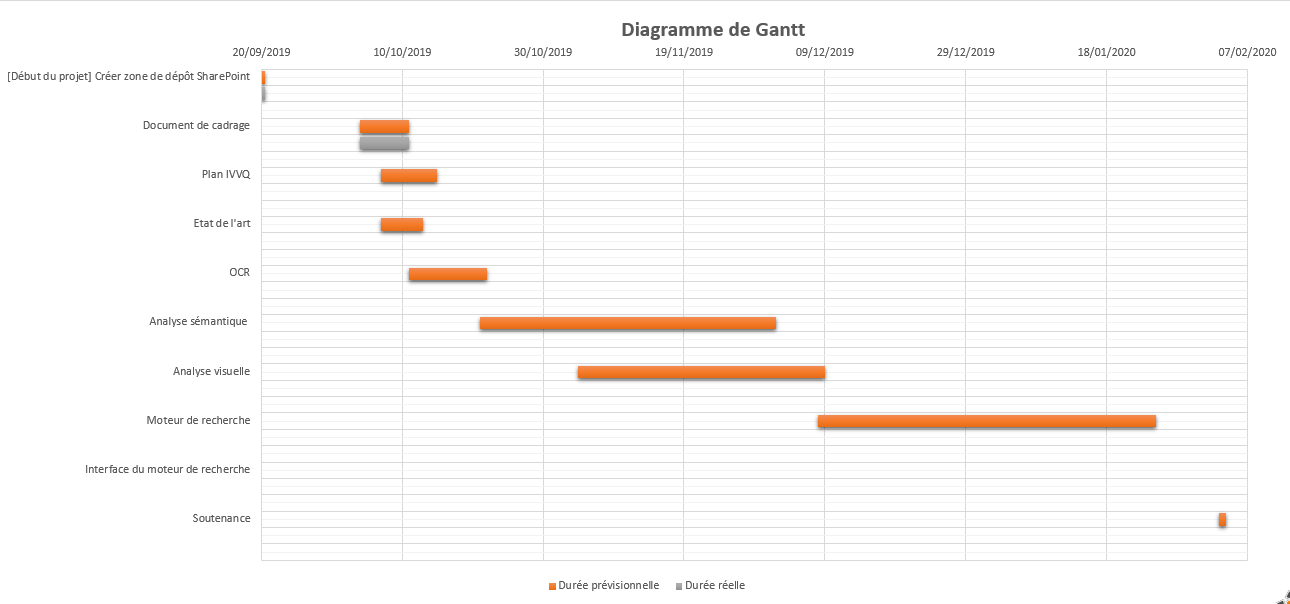
\includegraphics[width=\linewidth]{images/gantt.png}
	\caption{Gantt prévisionnel et post mortem}
	\label{fig:MC}
\end{figure}		

\section {Gouvernance}
%réunions, échanges, lieux de travail
\import {sections/} {fonctionnement}

\newpage
\end {document}

